%
% $RCSfile: first_trial.tex,v $
%
% Copyright (C) 2002-2008. Christian Heller.
%
% Permission is granted to copy, distribute and/or modify this document
% under the terms of the GNU Free Documentation License, Version 1.1 or
% any later version published by the Free Software Foundation; with no
% Invariant Sections, with no Front-Cover Texts and with no Back-Cover
% Texts. A copy of the license is included in the section entitled
% "GNU Free Documentation License".
%
% http://www.cybop.net
% - Cybernetics Oriented Programming -
%
% http://www.resmedicinae.org
% - Information in Medicine -
%
% Version: $Revision: 1.1 $ $Date: 2008-08-19 20:41:06 $ $Author: christian $
% Authors: Christian Heller <christian.heller@tuxtax.de>
%

\subsection{First Trial}
\label{first_trial_heading}
\index{EHR}
\index{Java}
\index{Graphical User Interface}
\index{GUI}
\index{MVC}
\index{Hierarchical MVC}
\index{HMVC}
\index{Composition}
\index{Res Medicinae with Nested Views}
\index{Object Oriented Programming}
\index{OOP}
\index{Topological Documentation in Res Medicinae}
\index{Res Medicinae Topological Documentation}

An early trial of a \emph{Res Medicinae} module was \emph{Record}, an application
for EHR management (figure \ref{record_figure}). It was a standard Java-based
system and had a \emph{Graphical User Interface} (GUI). Its classical
architecture made use of many software patterns (section \ref{pattern_heading})
and was shared into the parts \emph{Domain Model}, \emph{Graphical View} and
\emph{Controller}, as proposed by the equally named pattern, abbreviated
\emph{MVC}.

\begin{figure}[ht]
    \begin{center}
        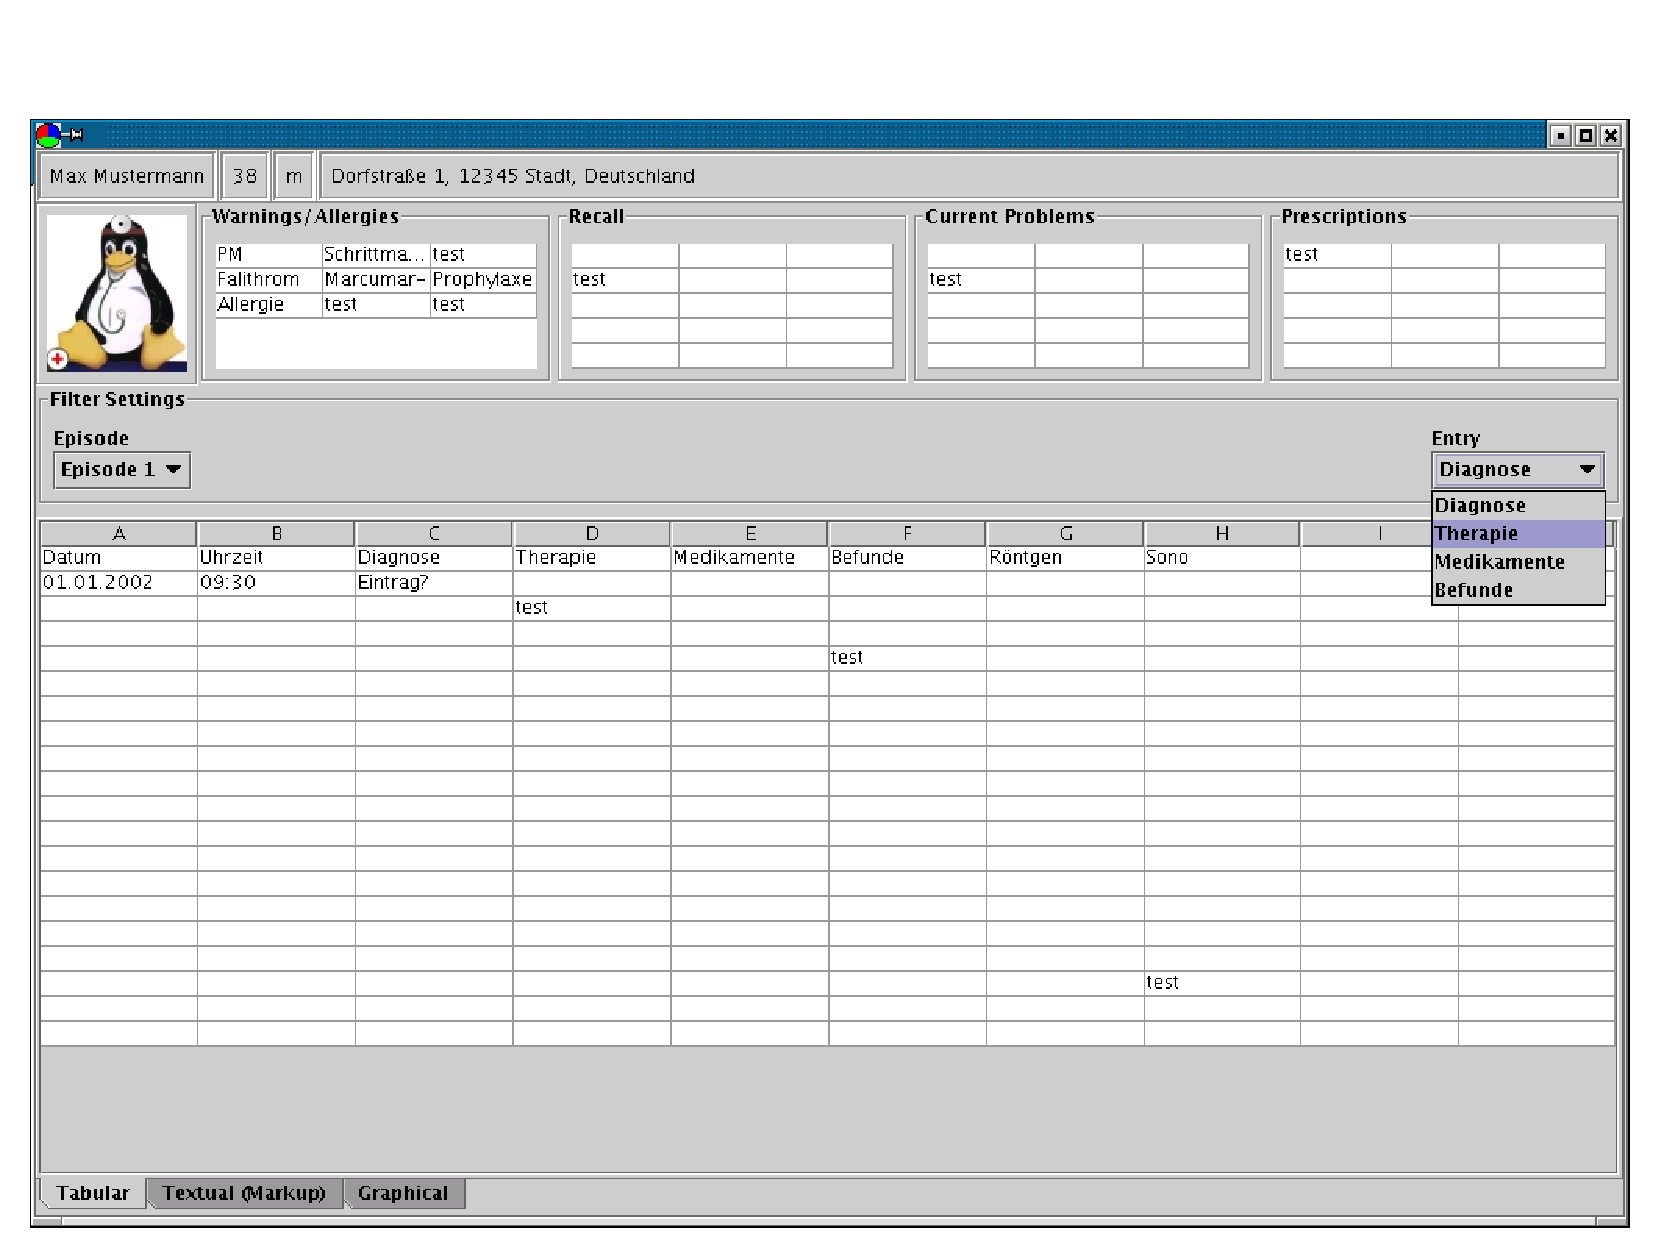
\includegraphics[scale=0.3,angle=-90]{graphic/record.pdf}
        \caption{Early Record Module}
        \label{record_figure}
    \end{center}
\end{figure}

Later prototypes extended that architecture by applying the CYBOP concept of
\emph{Composition}. In a first step, the \emph{Hierarchical MVC} (HMVC) pattern
was used to replace the MVC pattern, resulting in nested \emph{Controllers} and
\emph{Views} (figure \ref{frames_figure}). Afterwards, the principle of
\emph{Hierarchy} was applied in general, also to \emph{Domain Models} and to as
many other parts as possible.

\begin{figure}[ht]
    \begin{center}
        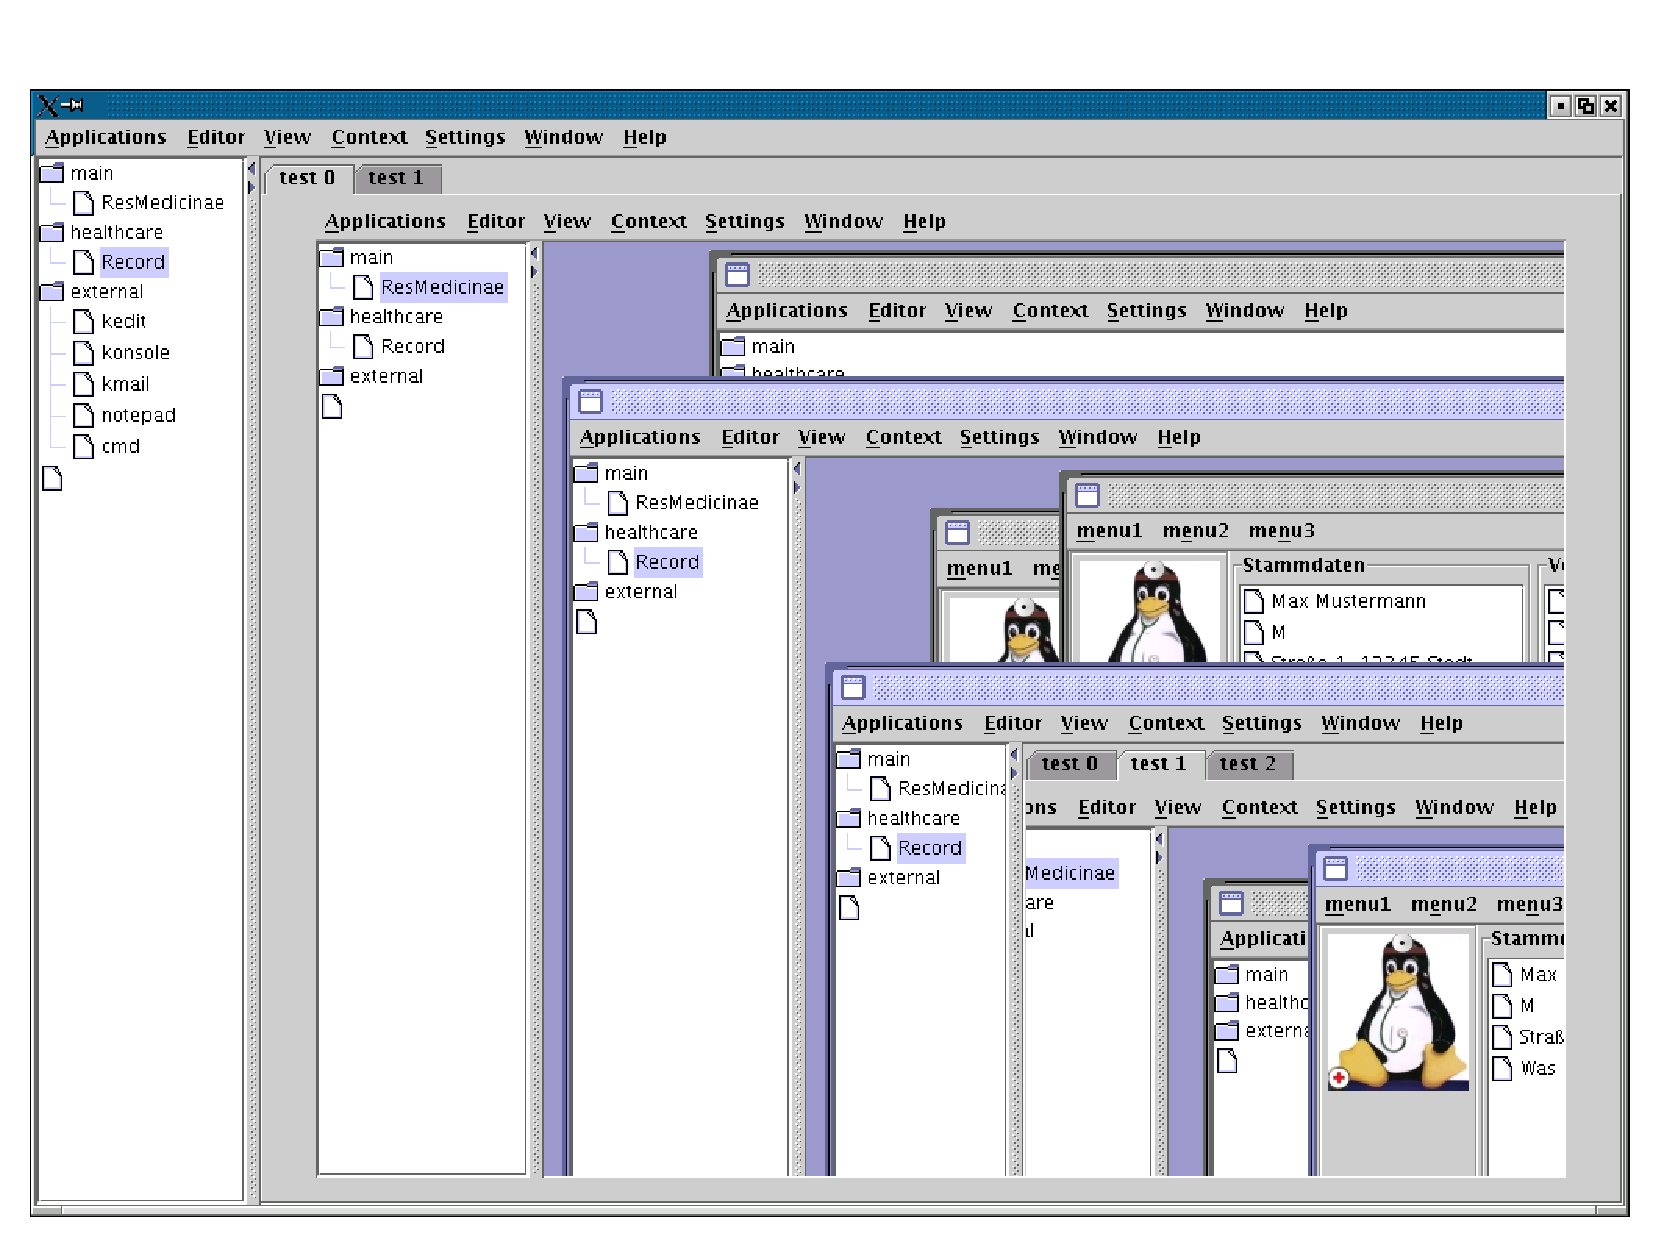
\includegraphics[scale=0.3,angle=-90]{graphic/frames.pdf}
        \caption{Nested Views of Module Frames}
        \label{frames_figure}
    \end{center}
\end{figure}

Classes as known from \emph{Object Oriented Programming} (OOP) do not represent
dynamically extensible containers but have a static structure with a fixed
number of attributes. In other words, the \emph{Hierarchy} as concept is not
inherent in OOP types. Yet abstract models as humans build them in their minds
are always based on hierarchies (section \ref{abstraction_heading}). A
programming language which does not consider this, does not allow users to make
full use of their modelling potential.

To eliminate this flaw and implement a hierarchical structure in the Java
prototype, a top-most super class named \emph{cybop.Model} had to be introduced
(compare also figure \ref{hashmap_figure}). It represented a container that had
the capability to reference itself -- in other words a \emph{Tree Structure}.
As such, it offered \emph{set}, \emph{get} and \emph{remove} methods for its
elements. Since these access methods were inherited, sub classes did not have
to implement their own (for each attribute) anymore, which saved hundreds of
lines of source code.

\begin{figure}[ht]
    \begin{center}
        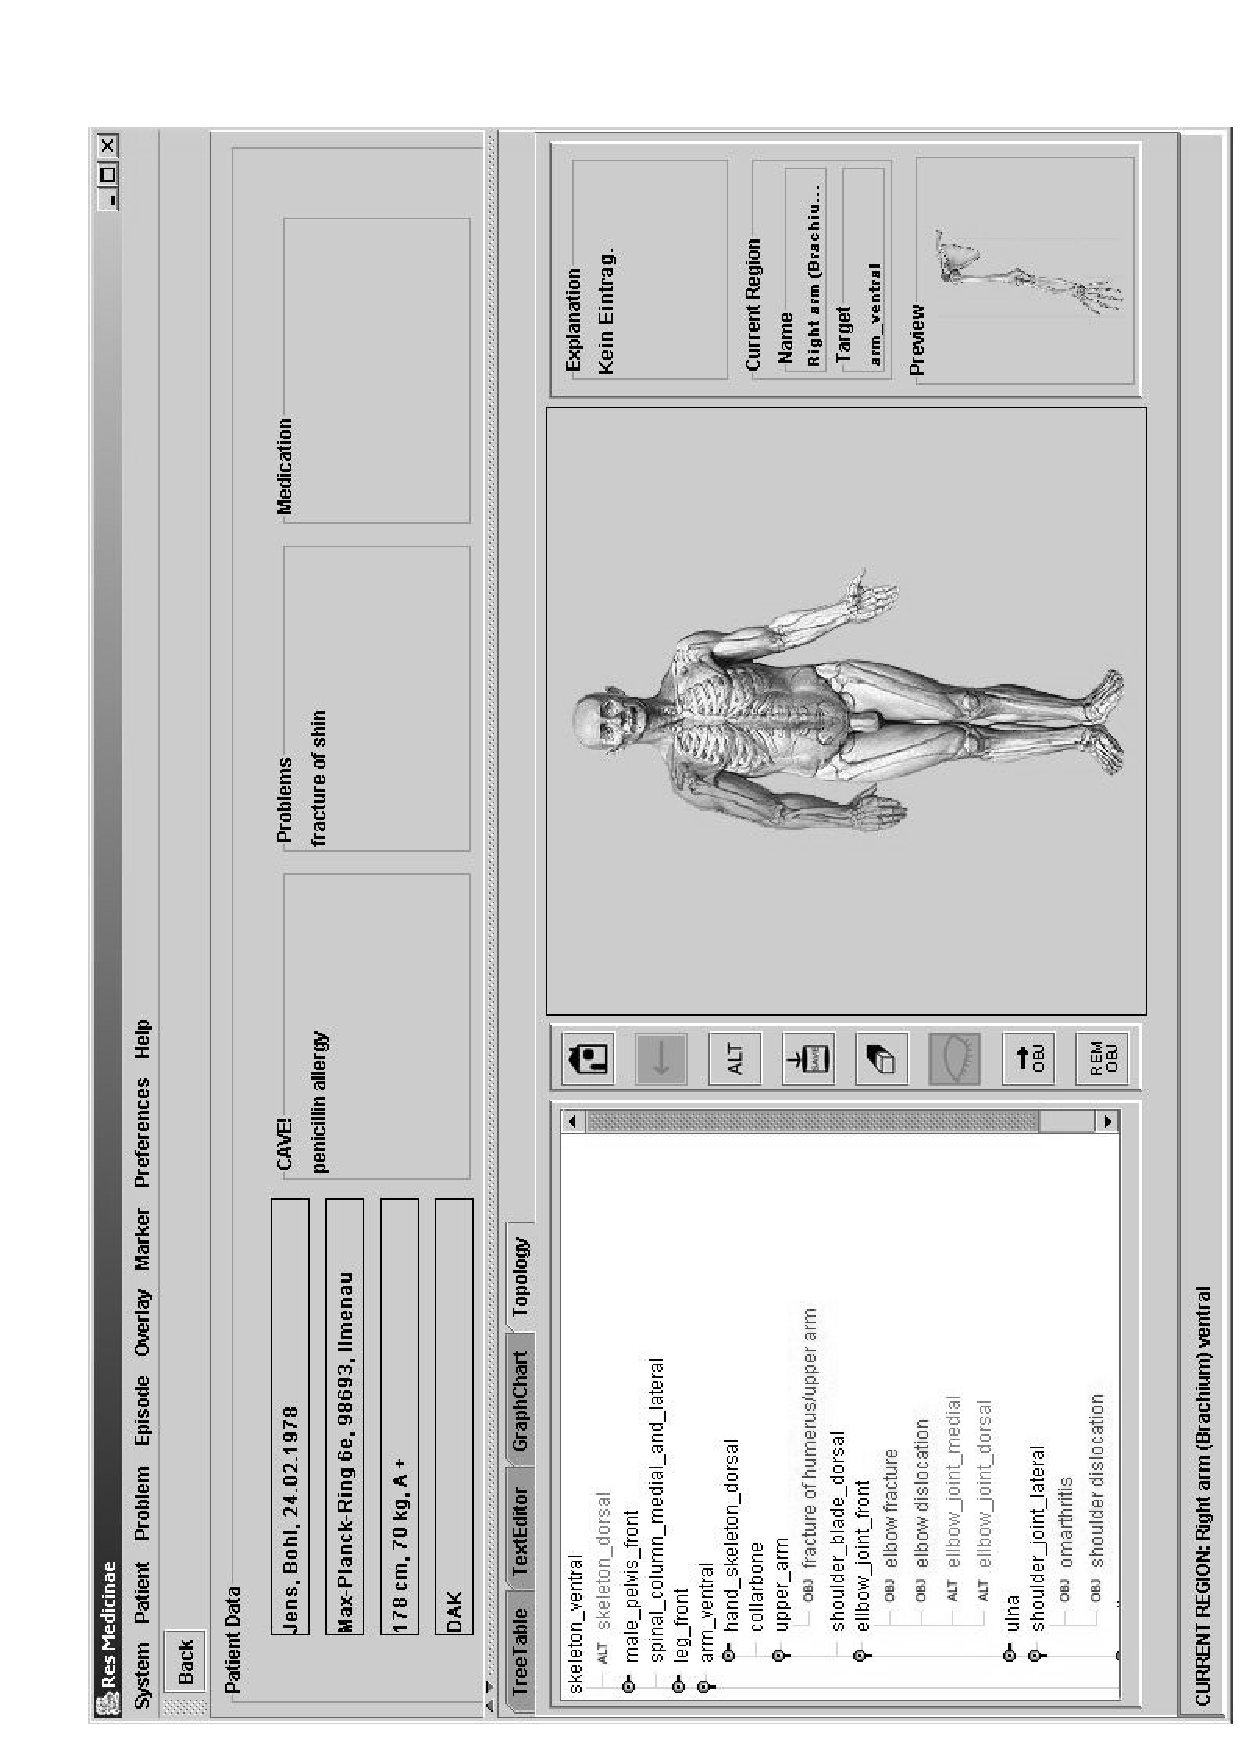
\includegraphics[scale=0.3,angle=-90]{graphic/topological.pdf}
        \caption{Topological Documentation in Record Module \cite{bohl}}
        \label{topological_figure}
    \end{center}
\end{figure}

One of these advanced modules (\emph{ReForm}) assisted medical form printing
\cite{kunze2003}, another one (\emph{ResAdmin}) managed administrative data of
patients with emphasis on internationalisation \cite{kanagasabapathi}, yet
another one (\emph{ResData}) served as appointment and scheduling module,
accessible over web \cite{holzmueller2005}, a backup application (\emph{Restore})
was implemented as well \cite{behrendt} and a last module (\emph{Record}, in an
extended version) was responsible for clinical documentation \cite{bohl}. This
documentation process was supported graphically, by \emph{Record's} ability for
\emph{Topological Documentation} (figure \ref{topological_figure}) and, of
course, it could also manage and store patient data, in XML files.
